\documentclass{report}

\usepackage[ngerman]{babel}
\usepackage[utf8]{inputenc}
\usepackage[T1]{fontenc}
\usepackage{hyperref}
\usepackage{graphicx}
\usepackage[german=guillemets]{csquotes}
\usepackage[a4paper]{geometry}
\usepackage{tikz}


\usepackage[
    backend=biber,
    style=apa,
    sortlocale=de_DE,
    natbib=true,
    url=false,
    doi=false,
    sortcites=true,
    sorting=nyt,
    isbn=false,
    hyperref=true,
    backref=false,
    giveninits=false,
    eprint=false]{biblatex}
\addbibresource{../references/bibliography.bib}


\title{Künstliche Intelligenz und deren Auswirkung auf die Arbeitswelt}
\author{Loïc Schneider}
\date{\today}


\begin{document}

\begin{titlepage}
    \makeatletter
    \begin{center}
        {\scshape Gymnasium Muttenz} \vspace{0.5cm}

        Informatik 2024\vspace{3.5cm}

        {\huge\bfseries \@title}

        \vspace{2cm}

        {\Large\bfseries Welche Chancen und Risiken bietet KI beim Einsatz in der Medizin?}

        \vspace{3cm}

        {\Large\itshape \@author}

        \vspace{0.5cm}

        Version vom: \@date

    \end{center}
    \makeatother

    % Ensure the image covers the entire page width and bottom margin
    \begin{tikzpicture}[remember picture,overlay]
        \node[anchor=south west,inner sep=0pt] at (current page.south west) {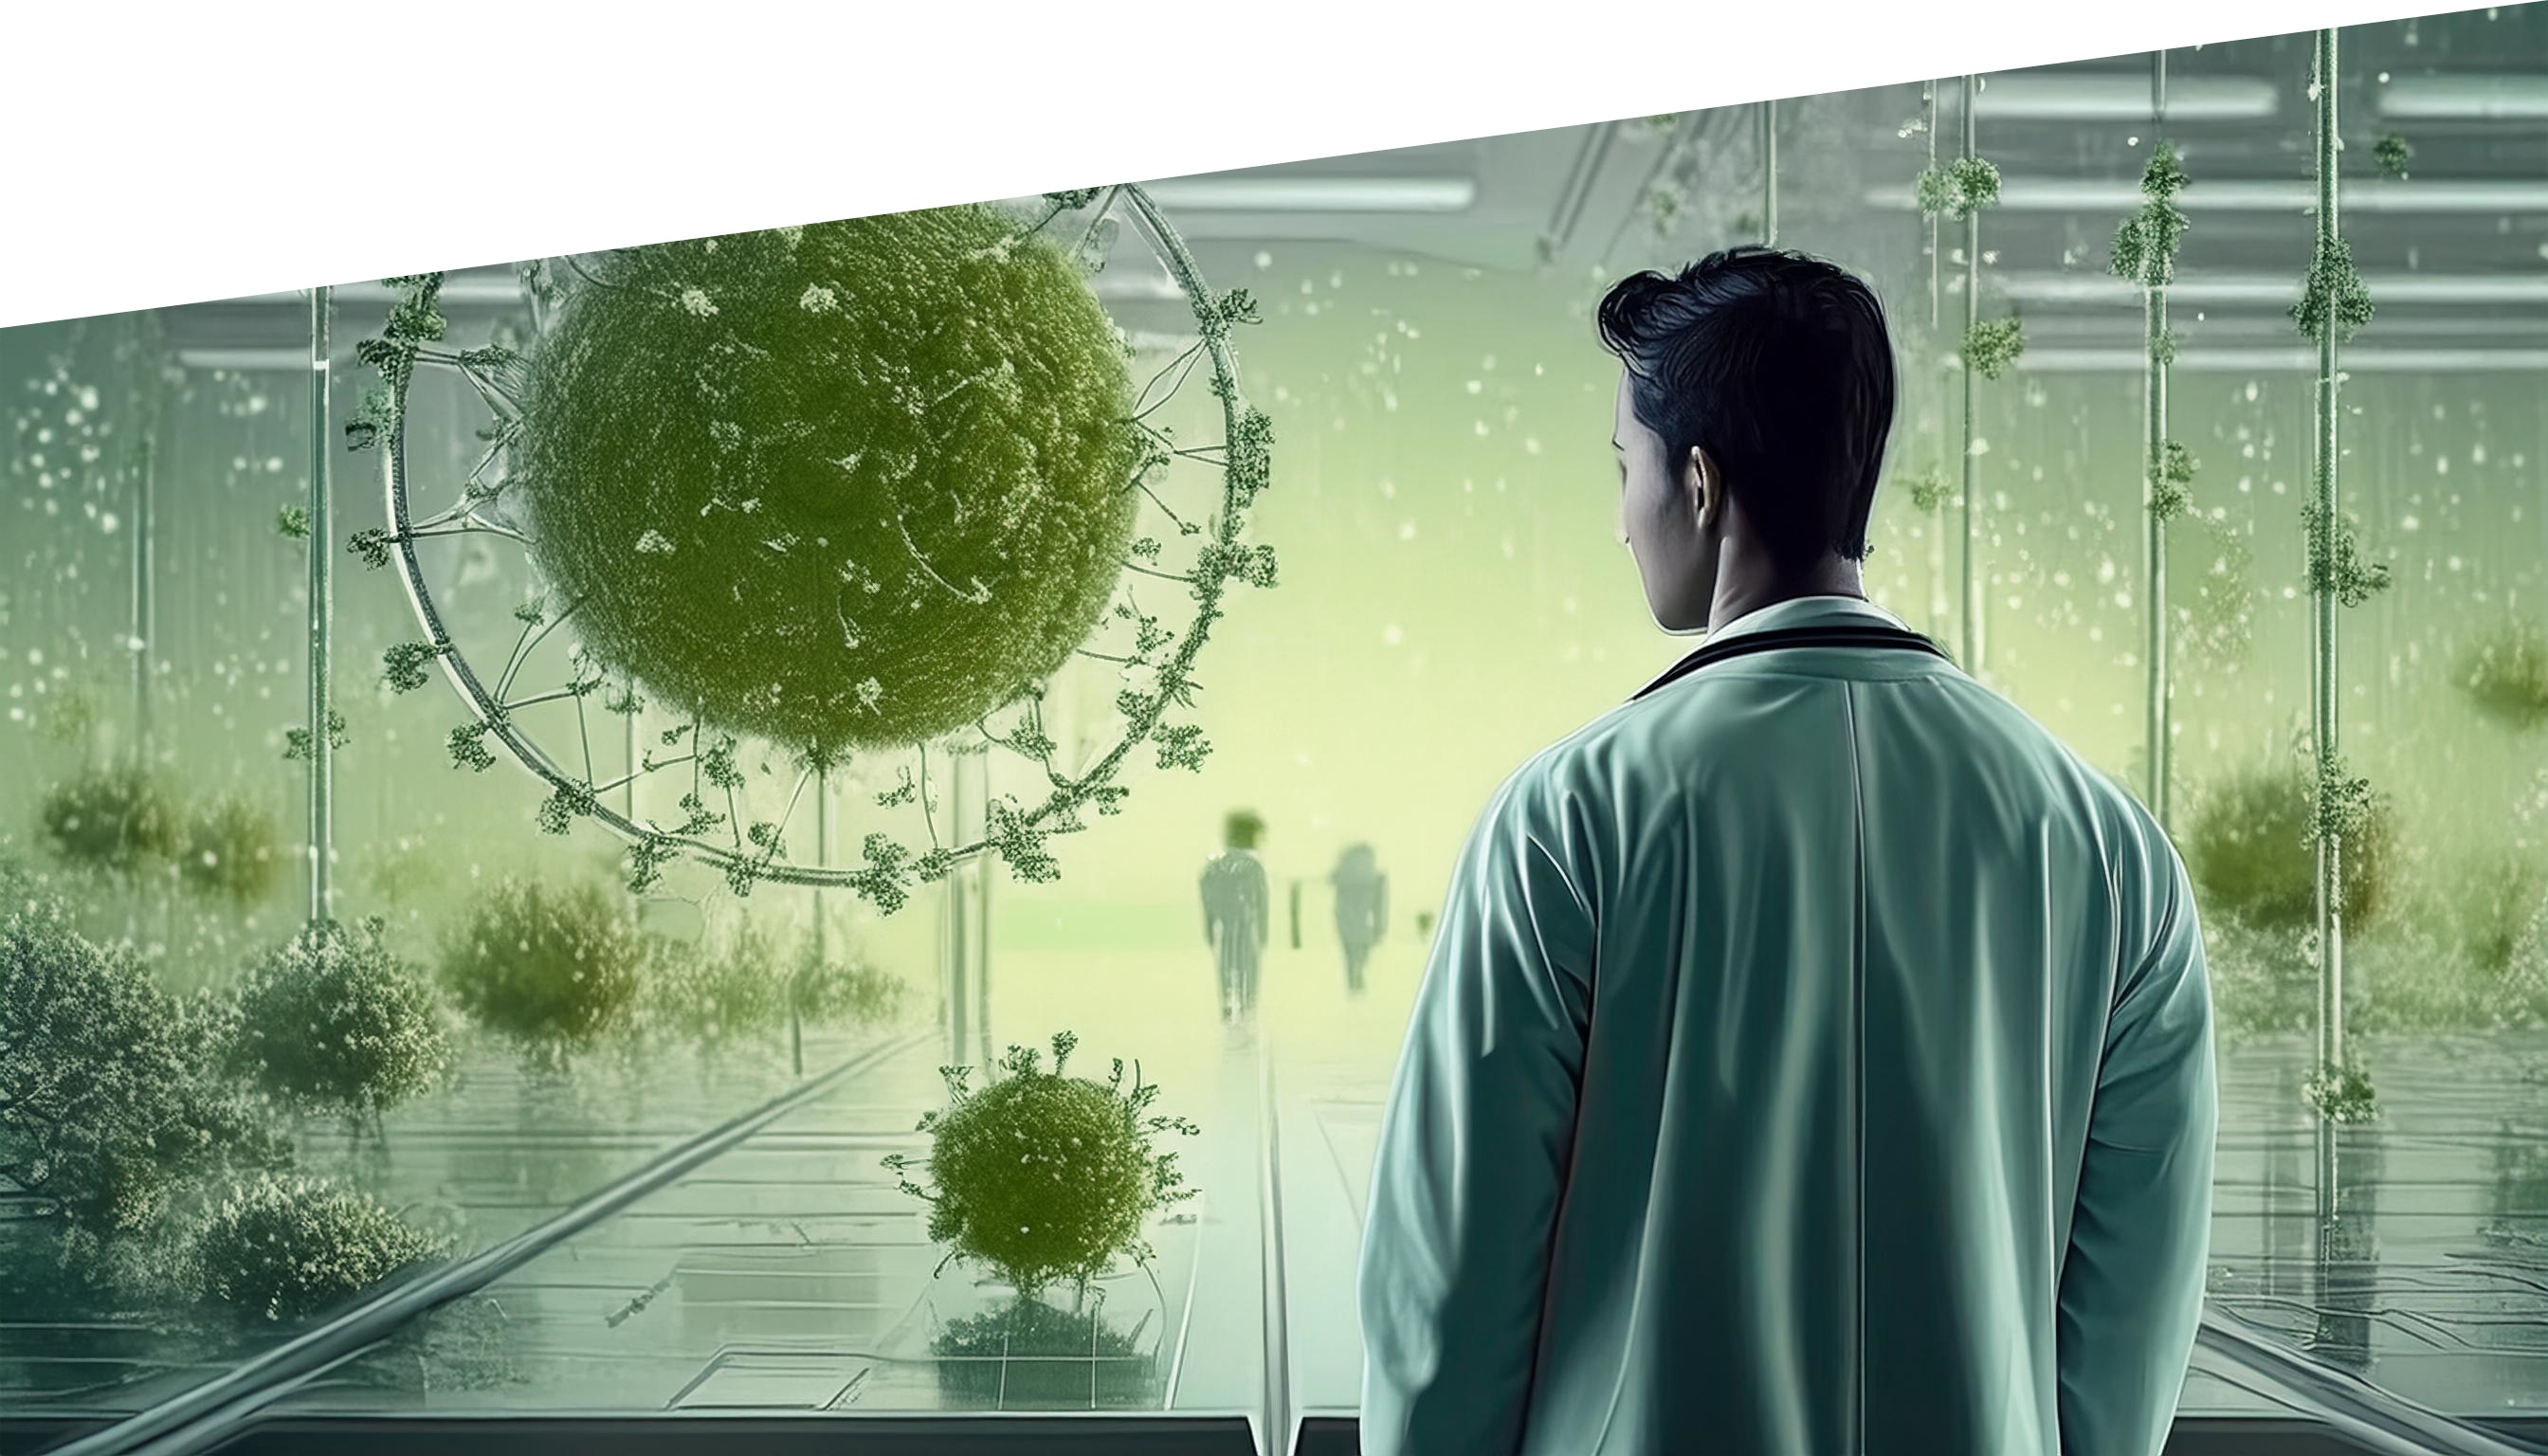
\includegraphics[width=\paperwidth, height=\paperheight, keepaspectratio]{TitlePicture.jpg}};
    \end{tikzpicture}
\end{titlepage}

\tableofcontents

\chapter{Einleitung}
\label{chap:introduction}

\enquote{Künstliche Intelligenz} ist heutzutage in jedermanns Munde. 
In den letzten Jahren hat sich die Technik rund um dieses Thema stark weiter entwickelt.
Während KI lange Zeit nur versteckt implementiert war und man sie als Nutzer oft garnicht bewusst wargenommen hat, wurde einem deren existenz aber spätestens durch die ganzen \enquote{Large Language Models} (LLMs) wie ChatGPT oder LaMDA vor Augen geführt.

Durch die sich stehts verbessernden Technologien hinter den KIs werden deren Anwenungsbereiche immer grösser.
Daher ist es nicht weit her geholt, dass KI dem Menschen gewisse Prozesse erleichtern oder abnehmen kann. 

In dieser Arbeit soll es genau um dieses Thema gehen. Wie sieht ein Berufsumfeld aus, wenn KI Technologien vermehrt Arbeiten des Menschen übernimmt und welche Chancen aber auch Risiken bringt dies mit sich.

\chapter{Wie lernt KI?}
\label{chap:ai-training}

Um alle Sachverhalte zu verstehen muss zuerst die Frage, wie eine KI erstellt, bzw. trainiert wird, geklärt werden.


\chapter{KI an Arbeitsplätzen}
\label{chap:ai-workingplaces}

Durch die steigenden technologischen Fähigkeiten von Maschinen durch KI, werden auch stetig neue Anwendungsbereiche geschaffen.
Auch in der Arbeitswelt nimmt KI einen grossen Einfluss. Immer mehr Arbeiten die zuvor noch von Menschen durchgeführt werden mussten, können durch Maschinen übernommen werden.
Damit verbunden steht das Risiko, dass Arbeitsplätze der automatisierung zum Opfer fallen könnten.
Trozdem gibt es viel Potential für Verbesserungen durch solche Technologien. Darunter sind zum Beispiel körperliche Entlastung oder erhöhte Sicherheitsstandarts.

Verbunden mit solchen änderungen sind viele Überlegungen. Beispielsweise müssen manche Arbeitsprofile angepasst werden, an anderen Stellen entstehrn vielleicht komplett neue.
KI gebundene System könnten unter den richtigen Umständen helfen Entscheidungen rationaler zu treffen und dadurch niemanden zu benachteiligen. 
Gleichzeitig taucht aber auch der kritische Punkt des Datenschutzes von verschiedenen Parteien wie Arbeitnehmer*innen, Empfänger*innen von Dienstleistungen oder Ähnlichem auf.

Daran, dass digitale Technologien wie KI Veränderungen in die Arbeitswelt bringen werden oder es auch schon tun, ist kein Zweifel.
Es gilt aber, sich viele Gedanken um Themen wie den Datenschutz, Entscheidungsbeschränkung oder gesetzlichen Vorlagen zu KIs zu machen.

\chapter{KI in der Medizin}
\label{chap:ai-medicine}

Ein grosses potenzielles und auch teilweise schon exisiterendes Anwendungsgebiet für Künstliche Intelligenzen liegt in der Medizin.
Dort kann diese vielseitig, beispielsweise für Diagnosen oder eine Ersteinschätzung von Patienten eingesetzt werden.

Dabei entstehen grosse Chancen wie aber auch Risiken.

\section{Chancen}
Dem vermehrten Einsatz von KI in der Bedizin stehen viele Chancen gegenüber.
Ein Problem in der Medizin ist, dass sich Ärtze zu wenig Zeit nehmen können um wirklich auf die Patienten einzugehen und eine Verbindung aufzuabauen.
Wenn KI gewisse Aufgaben übernehmen kann, würde das die Ärtzte entlasten und sie könnten sich wieder verstärkt auf die Patienten einlassen, was den Arbeitsaltag der Ärtze erleichtert so wie dem Patienten ein besseeres Gefühl zu vermitteln.


\section{Risiken}

\chapter{Fazit}
\label{chap:Fazit}

Die Integration von Künstlicher Intelligenz in die Medizin bietet sowohl immense Chancen als auch erhebliche Risiken. 

KI kann die Medizin effizienter, präziser und patientenorientierter gestalten, indem sie Ärzte entlastet und durch ihre Fähigkeit die Diagnose und Behandlung von Krankheiten verbessert. 
Zudem kann KI die Forschung nach neuen Medikamenten und Behandlungsmethoden unterstützen und durch Fernüberwachung oder virtuelle Assistenten Patienten auch außerhalb von medizinischen Einrichtungen helfen.

Dennoch sind diese Vorteile nicht ohne Herausforderungen. Ethische Bedenken, Datenschutzfragen und die Zuverlässigkeit der KI-Systeme stellen bedeutende Risiken dar. 
Die Skepsis der Patienten gegenüber der Sicherheit und Funktionalität der KI kann zu einer Ablehnung von Behandlungen führen, was wiederum physische und psychische Folgen haben kann. 
Der Umgang mit sensiblen Patientendaten erfordert strikte Datenschutzmaßnahmen.
Ethische Überlegungen betreffen die Frage, wie viel Verantwortung an Maschinen abgegeben werden sollte, die letztlich auf algorithmischen Entscheidungen basieren und keine moralische Urteilsfähigkeit besitzen. 
Rechtliche Fragen zur Haftung im Falle von Fehlern durch KI-Systeme müssen geklärt werden, und es ist wichtig, dass Entscheidungen, die von KI getroffen werden, für Ärzte und Patienten nachvollziehbar sind.

\vspace{5mm} \noindent
Insgesamt muss der Einsatz von KI in der Medizin sorgfältig geplant und überwacht werden, um sicherzustellen, dass die Vorteile maximiert und die Risiken minimiert werden. 
Datenschutz, ethische Prinzipien und rechtliche Rahmenbedingungen müssen dabei stets berücksichtigt werden, um den sicheren und verantwortungsvollen Einsatz von KI in der Gesundheitsversorgung zu gewährleisten.


\nocite{*}

\printbibliography

\end{document}
